\documentclass[11pt,oneside]{uhthesis}
%\documentclass[11pt,oneside]{report}
\usepackage{subfigure}
\usepackage[linesnumbered,lined,titlenumbered,ruled,algochapter,spanish,onelanguage]{algorithm2e}


\usepackage{substr}
\usepackage{bbm}
\usepackage{lipsum}
%\usepackage{easyReview}

\usepackage{amsmath}
\usepackage{theorem}
\usepackage{amssymb}
\usepackage{amsbsy}
%\usepackage{mathpazo}


\usepackage{float}
\usepackage{braket}
\usepackage[htt]{hyphenat}
\setlength {\marginparwidth }{3cm}


\usepackage[spanish]{babel}
\usepackage{graphicx}

\usepackage{listings}
\usepackage{color}
\usepackage{booktabs}
\usepackage{multirow}
\usepackage{ragged2e}
\usepackage{multicol}
\usepackage{comment} 

\usepackage{hyphenat}
\hyphenation{in-te-rac-tú-an}

\spanishdecimal{.}

\floatstyle{ruled}
\restylefloat{table}
\usepackage{color}

\usepackage[disable]{todonotes}

\definecolor{dkgreen}{rgb}{0,0.6,0}
\definecolor{gray}{rgb}{0.2,0,0}
\definecolor{mauve}{rgb}{0.58,0,0.82}

\lstset{language=Python,
	aboveskip=10mm,
	belowskip=10mm,
	showstringspaces=false,
	columns=flexible,
	basicstyle={\small\ttfamily},
	keywordstyle=\color{blue},
	commentstyle=\color{dkgreen},
	stringstyle=\color{mauve},
	breaklines=true,
	breakatwhitespace=true,
	tabsize=3,
	numbers=left, numberstyle=\tiny, stepnumber=1,firstnumber=1,
	numbersep=5pt
}

\renewcommand{\tablename}{Tabla}
\title{Textos alternativos para las colecciones de imágenes del repositorio digital de la Oficina  del historiador de La Habana}
\author{\\Amanda Cordero Lezcano\\ Ana Paula González Muñoz\\ Carlos Antonio Bresó Sotto\\ Christopher Guerra Herrero\\ Dennis Daniel González Durán\\ Marian Susana Álvarez Suri}

\faculty{Facultad de Matemática y Computación}
\date{Enero 2025}
\logo{Graphics/uhlogo}

\renewcommand{\vec}[1]{\boldsymbol{#1}}
\newcommand{\diff}[1]{\ensuremath{\mathrm{d}#1}}



\newcommand{\correccion}[2][noinline]{\todo[backgroundcolor=pink,linecolor=pink,#1]{\scriptsize {#2}}}



% Para definir teoremas, lemas, definiciones, corolarios, pruebas

\newtheorem{definicion}{Definición}
\newtheorem{lema}{Lema}
\theoremstyle{break}
\newtheorem{teorema}{Teorema}
\theoremstyle{break}
\newtheorem{corolario}{Corolario}[teorema]
\newtheorem{prueba}{Prueba}
%\theoremstyle{break}

% Para citar teoremas, lemas, definiciones, corolarios, pruebas
\newcommand{\reftheorem}[1]{\IfBeforeSubStringEmpty{teorema}{#1}{\textbf{Teorema~\ref{#1}}}{\IfBeforeSubStringEmpty{lema}{#1}{\textbf{Lema~\ref{#1}}}{\IfBeforeSubStringEmpty{prueba}{#1}{\textbf{Prueba~\ref{#1}}}{\IfBeforeSubStringEmpty{corolario}{#1}{\textbf{Corolario~\ref{#1}}}{\IfBeforeSubStringEmpty{definicion}{#1}{\textbf{Definición~\ref{#1}}}{{\color{red} Citado Erróneo}}}}}}}

\newcommand{\reftheorempage}[1]{\IfBeforeSubStringEmpty{teorema}{#1}{\textbf{Teorema~\ref{#1}} (pág \pageref{#1})}{\IfBeforeSubStringEmpty{lema}{#1}{\textbf{Lema~\ref{#1}} (pág \pageref{#1})}{\IfBeforeSubStringEmpty{prueba}{#1}{\textbf{Prueba~\ref{#1}} (pág \pageref{#1})}{\IfBeforeSubStringEmpty{corolario}{#1}{\textbf{Corolario~\ref{#1}} (pág \pageref{#1})}{\IfBeforeSubStringEmpty{definicion}{#1}{\textbf{Definición~ \ref{#1}} (pág \pageref{#1})}{{\color{red} Citado Erróneo}}}}}}}

\begin{document}
\selectlanguage{spanish}

%\frontmatter
\maketitle

\begin{abstract}
	{\small
	Se presenta un sistema de generación de textos alternativos para imágenes del repositorio digital de la Oficina del Historiador de La Habana. Se exploraron modelos de aprendizaje profundo, incluyendo BLIP, Visual Transformers + GPT-2 y CLIP, para la genereación. Se realizó un análisis detallado del estado del arte, identificando modelos de redes recurrentes, convolucionales y basados en Transformers. La metodología combinó la generación de descripciones con un algoritmo de selección basado en similitud semántica. Los resultados fueron evaluados mediante métricas BLEU, METEOR, CIDEr, ROUGE, y SPICE.
}
\end{abstract}

\tableofcontents
%\listoffigures
%\listoftables


%\mainmatter
	
%===================================================================================
% Chapter: Introduction
%===================================================================================
\chapter{Introducción}\label{chapter:introduction}
%===================================================================================
En este proyecto, se desarrolla un sistema de generación de texto alternativo para las imágenes del repositorio digital de la Oficina del Historiador de la Ciudad de La Habana. Creando descripciones precisas y detalladas que mejoren la accesibilidad a la información, permitan una mejor búsqueda y recuperación de imágenes. 

El problema de generar texto alternativo para imágenes ha sido abordado mediante el uso de técnicas avanzadas de procesamiento del lenguaje natural (NLP) y visión por computadora. Investigaciones recientes han utilizado redes neuronales convolucionales (CNN) para analizar y comprender el contenido visual de las imágenes, combinadas con redes neuronales recurrentes (RNN) o Transformers para generar descripciones textuales coherentes y contextualmente adecuadas. Estos modelos han demostrado ser efectivos en la tarea de generación de texto alternativo, permitiendo la creación automática de descripciones.

La propuesta de solución implica la combinación de dos modelos pre-entrenados de generación de texto alternativo, con los cuales se generan dos descripciones para cada imagen, y luego se aplica un algoritmo de selección que elige la descripción que mejor se ajusta a cada imagen específica. Esta metodología no solo aprovecha las capacidades avanzadas de cada modelo, sino que también asegura que la descripción final sea la más precisa y relevante.
 
%===================================================================================
% Chapter: Estado del Arte
%===================================================================================
\chapter{Estado del Arte}\label{chapter:estadoarte}
%===================================================================================

El campo del \textit{image captioning} ha evolucionado significativamente en la última década, impulsado por el avance de modelos de aprendizaje profundo. En este capítulo, se presentan los principales enfoques y modelos que han marcado hitos en esta área, destacando sus arquitecturas, metodologías y contribuciones.

\section{Modelos Basados en Redes Recurrentes}

Los primeros avances en generación de descripciones de imágenes se apoyaron en arquitecturas \textit{encoder-decoder} con redes neuronales recurrentes (RNN). Uno de los primeros modelos destacados fue \textbf{Show and Tell} \cite{vinyals2015show}, que utilizó una combinación de una red convolucional (CNN) para la extracción de características visuales y una red LSTM para la generación de texto. Este modelo logró buenos resultados en datasets como MSCOCO y Flickr30k, evaluándose con métricas como BLEU y METEOR.

Posteriormente, \textbf{Show, Attend and Tell} \cite{xu2015show} introdujo mecanismos de atención visual, permitiendo que el modelo enfocara diferentes regiones de la imagen en cada paso de generación. Este enfoque mejoró la calidad de las descripciones y presentó una formulación matemática más avanzada para el cálculo de la atención.

\section{Modelos Basados en Redes Convolucionales}

En un intento por superar las limitaciones de las RNN, \textbf{Convolutional Image Captioning} \cite{aneja2018convcap} propuso una arquitectura basada en CNNs para la generación de texto. Este modelo demostró que las CNNs pueden superar a las LSTM en tareas de \textit{captioning}, especialmente cuando se combinan con mecanismos de atención, mitigando problemas como el desvanecimiento del gradiente.

\section{Atención y Modelos Jerárquicos}

Otro enfoque relevante fue el modelo \textbf{Bottom-Up and Top-Down} \cite{anderson2018bottom}, que implementó un mecanismo de atención jerárquico basado en la segmentación de objetos dentro de la imagen. Este modelo mejoró el rendimiento en tareas como \textit{Visual Question Answering} e \textit{image captioning}, utilizando datasets como Visual Genome y MSCOCO.

\textbf{Knowing When to Look} \cite{lu2017knowing} propuso un mecanismo de atención adaptativo mediante un centinela visual, que decide cuándo prestar atención a la imagen y cuándo confiar en el contexto textual generado previamente. Este modelo ofreció mejoras en métricas como CIDEr y BLEU.

\section{Transformers y Modelos Multimodales}

Con la llegada de los Transformers, los modelos de \textit{captioning} han adoptado arquitecturas más avanzadas. \textbf{Multimodal Transformer} \cite{yu2019multimodal} exploró la representación visual multi-vista para mejorar la generación de texto, mientras que \textbf{BLIP} \cite{li2022blip} amplió la capacidad de los modelos al abordar tanto la generación como la comprensión de imágenes y videos, logrando mejoras en tareas como recuperación de imágenes y preguntas visuales.

Además, \textbf{CLIP} \cite{radford2021learning} introdujo el aprendizaje multimodal a gran escala utilizando correspondencias entre imágenes y texto en internet, mientras que \textbf{ViT} \cite{dosovitskiy2021image} aplicó Transformers directamente a imágenes dividiéndolas en parches, lo que representó un cambio significativo en el procesamiento de información visual.

\section{Resumen y Tendencias Actuales}

La evolución del \textit{image captioning} ha pasado de modelos basados en RNNs con atención visual a enfoques más sofisticados que integran Transformers y aprendizaje multimodal. Modelos recientes como BLIP y CLIP han demostrado que la combinación de visión y lenguaje en grandes volúmenes de datos puede llevar a mejoras sustanciales en la generación y comprensión de imágenes. 

Las tendencias actuales apuntan a modelos más eficientes y escalables, con capacidades mejoradas en la generación de texto y una mayor comprensión del contexto visual. El impacto de estas tecnologías se extiende más allá del \textit{image captioning}, beneficiando tareas como búsqueda visual, generación de contenido y asistencia en accesibilidad.



%===================================================================================
% Chapter: Introduction
%===================================================================================
\chapter{Propuesta}\label{chapter:propuesta}
%===================================================================================
Se propone un sistema para la generación de texto alternativo a partir de las imágenes del repositorio digital del patrimonio cultural de la Oficina del Historiador, combinando múltiples modelos de aprendizaje profundo. La metodología se basa en un enfoque de evaluación comparativa entre diferentes modelos de generación de texto a partir de imágenes, utilizando un criterio de selección basado en la similitud semántica con el contenido visual.

En primer lugar, se emplea el modelo BLIP (Bootstrapped Language-Image Pretraining) para generar una primera descripción de la imagen. Posteriormente, la imagen es procesada por el modelo ViT (Vision Transformer) en conjunto con GPT-2, obteniendo una segunda descripción independiente. Finalmente, el modelo CLIP (Contrastive Language-Image Pretraining) se utiliza como mecanismo de selección, comparando las dos descripciones generadas y eligiendo la que presente una mayor correspondencia semántica con la imagen de entrada.

% TODO: \usepackage{graphicx} required
\begin{figure}
	\centering
	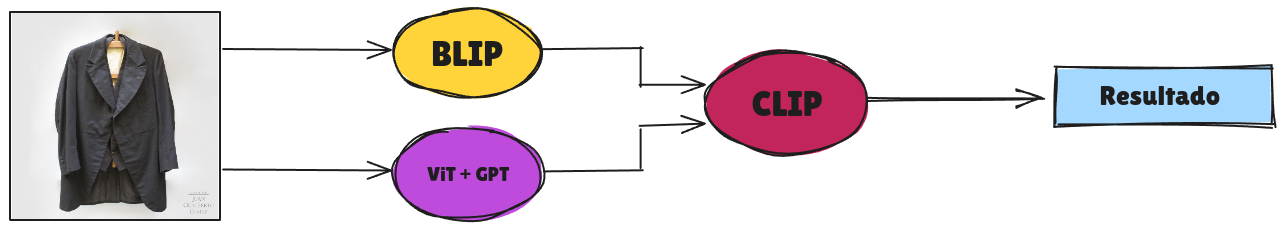
\includegraphics[width=1\linewidth]{./Graphics/diagrama}
	\caption{Modelo general}
	\label{fig:diagrama}
\end{figure}

%===================================================================================
% Chapter: Introduction
%===================================================================================
\chapter{Desarrollo de la propuesta}\label{chapter:desarrollo}
%===================================================================================
El primer paso en nuestro proyecto fue la descarga del dataset de imágenes desde el servidor.

Se realizó una investigación exhaustiva sobre el estado del arte en el campo de procesamiento de imágenes para generación de textos alternativos. El resumen incluyó una caracterización de las formas de aprendizaje en los modelos de Machine Learning, la arquitectura que se llevó a cabo para el desarrollo del algoritmo, el modelo de lenguaje empleado, así como los datasets y métricas que fueron seleccionados durante el entrenamiento y evaluación de los modelos. 

Se seleccionaron los modelos que mejor se adaptaban a nuestro caso, optando por BLIP y Visual Transformers (GPT-2), los cuales destacan por su eficacia en tareas de procesamiento de imágenes y generación de texto. 

Se realizó un análisis exploratorio de los datos para comprender mejor las características y peculiaridades del dataset, lo cual contribuyó a identificar patrones y posibles problemas que podrían ser enfrentados durante el procesamiento de las imágenes.

Se procesaron todas las imágenes localmente utilizando los modelos seleccionados y mediante el uso de CLIP, se seleccionó la descripción que mejor se adaptaba a cada imagen.

Utilizamos las métricas BLEU y METEOR sobre los resultados obtenidos para evaluar el rendimiento de nuestros modelos, lo que nos permitió medir la efectividad de nuestro enfoque.

Finalmente, analizamos estadísticas básicas sobre los resultados finales. Este análisis nos proporcionó una visión clara de la calidad y consistencia de nuestras descripciones generadas y nos ayudó a identificar áreas de mejora para futuros proyectos.

%===================================================================================
% Chapter: Introduction
%===================================================================================
\chapter{Resultados}\label{chapter:resultados}
%===================================================================================





%\backmatter
%===================================================================================
% Chapter: Conclusiones
%===================================================================================
\chapter{Conclusiones}\label{chapter:conclusions}




\renewcommand{\bibname}{Referencias}
% \nocite{*}
\bibliographystyle{unsrt}
\bibliography{Bibliography.bib}


\end{document}